\documentclass{beamer}
\usetheme[faculty=econ]{fibeamer}

\usepackage[utf8]{inputenc}
\usepackage[francais]{babel}
\usepackage[T1]{fontenc}
\usepackage{xcolor}

\lstset{
  language=Java,                
  basicstyle=\scriptsize,
  escapeinside={*@}{*@},
  frame=single,
  xleftmargin=2mm,
  xrightmargin=2mm,
  keepspaces=true,
  tabsize=2
}

\newcounter{ctr1}
\title[]{\Large{Développement d'applications modulaires en Java}}
\author[C. Tibermacine]{\large{Chouki~Tibermacine}\\
\small{Chouki.Tibermacine@umontpellier.fr}}
%\institute{Polytech Montpellier}
\date{}

\begin{document}

\begin{frame}
\titlepage
\begin{flushright}

\includegraphics[width=3.5cm]{figs/polytech.png}
\end{flushright}
\end{frame}

\begin{frame}
	\frametitle{Plan de l'ECUE}
	\begin{enumerate}
		{\color{gray}{\item (Rappels sur le) Développement d'applications Web avec Java
				\item Modulariser les applications Java avec Spring
				\item Bien structurer une application Web avec Spring MVC
				\item Auto-configurer une application Web avec Spring Boot
				\item Sécuriser une application Web avec Spring Security
				\item Gérer des données massives avec Apache Kafka et Spring
				\item Tester une application Web Spring}}			
				\item Écrire des applications Web (API) réactives avec Spring WebFlux

	\end{enumerate}
\end{frame}

\AtBeginSection[]{% Print an outline at the beginning of sections
  \begin{frame}<beamer>
    \frametitle{Plan du cours}
    % \frametitle{Outline}
    \tableofcontents[currentsection]
    % \tableofcontents
  \end{frame}}

\AtBeginSubsection[]{% Print an outline at the beginning of sections
  \begin{frame}<beamer>
    \frametitle{Plan du cours}
    % \frametitle{Outline}
    \tableofcontents[currentsubsection]
    % \tableofcontents
  \end{frame}}

\section{API \textit{Reactive Streams} et son implem \textit{Reactor}}
\begin{frame}
  \frametitle{Pourquoi une autre API pour les app Web~?}
  \textbf{Besoins en appels non-bloquants et asynchrones}
  \begin{itemize}
  \item L'API des servlets permet de créer des servlets synchrones
  \item Possibilité d'écrire des servlets asynchrones depuis l'API 3.1+ (vus dans le premier cours)
  \item Malgré cela, ce qui entoure ces servlets reste synchrone, comme les appels dans les filtres, ou bloquant comme les appels à \texttt{getParameter()}
  \item Besoin de gérer la concurrence (et la scalabilité) avec peu de ressources matérielles en utilisant une API asynchrone et non-bloquante
  \item Cela a été rendu possible grâce à des serveurs comme Netty
\end{itemize}
  \textbf{Besoins d'utiliser la programmation déclarative \& fonctionnelle}
  \begin{itemize}
  	\item Arrivée des annotations dans Java 5
  	\item Arrivée des lambdas et de l'API Stream dans Java 8
  \end{itemize}
\end{frame}

\begin{frame}
	\frametitle{Que veut dire ``programmation réactive"~?}
	\begin{itemize}
		\item Un modèle de programmation basé sur la réaction au changement~:
		\begin{itemize}
			\item Des composants en réseau réagissant aux entrées/sorties
			\item Des composants UI réagissant aux événements de la souris
		\end{itemize}
	\item Un programme est réactif $\Rightarrow$ il n'est pas bloqué
	\item Au lieu de rester bloqué (en attente d'une opération qu'elle se termine), il est prêt à réagir aux notifications et à la disponibilité des données
	\item Rien de nouveau : pattern \textit{publish-subsribe} (1 producteur de données et 1 souscripteur, qui est réveillé quand des données sont produites)
\end{itemize}
\end{frame}

\begin{frame}
\frametitle{\textit{Back Pressure}}
	\begin{tikzpicture}[overlay,remember picture]
		\node[anchor=center,xshift=0pt,yshift=20pt]
		at (current page.center) {
			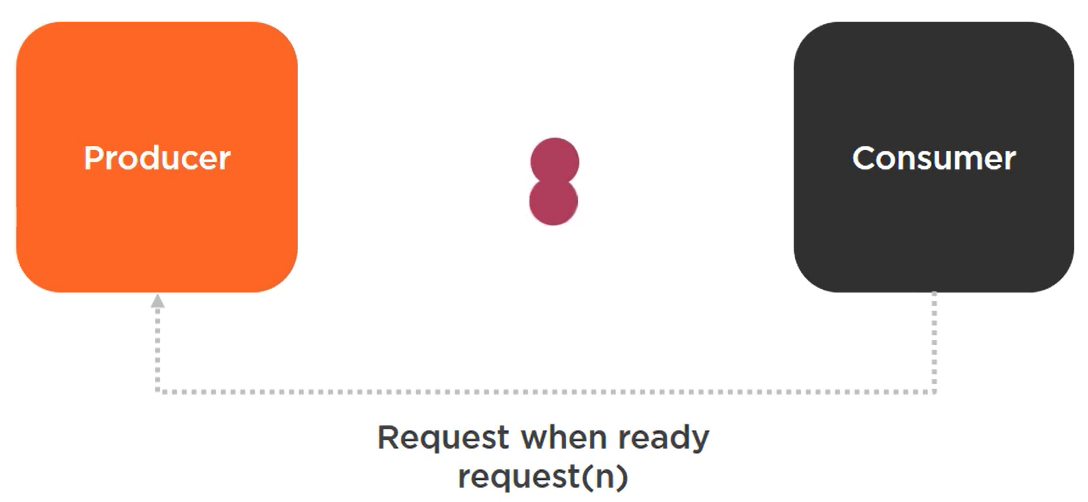
\includegraphics[width=10cm]{img/backpressure.png}
		};
	\end{tikzpicture}

\begin{itemize}	
	\vspace{4cm}
	\item Concept étroitement lié à la programmation réactive
	\item Il signifie le contrôle de la production de données pour que le souscripteur ne soit pas dépassé par le traitement des données qu'il reçoit du producteur
	\end{itemize}
\end{frame}

\begin{frame}
	\frametitle{\textit{Back Pressure} -suite-}
	Et si le producteur ne peut pas contrôler la production de données~?
	\begin{itemize}
		\item Il doit être capable de bufferiser les données, les ignorer ou s'arrêter
	\end{itemize}
	Ceci relève de l'applicatif et non du mécanisme des \textit{Reactive Streams}
\end{frame}

\begin{frame}
	\frametitle{Reactive Streams}
	\begin{itemize}
		\item Une API, adoptée dans Java 9, permettant d'écrire des composants asynchrones avec \textit{back pressure}
		\item Des composants \texttt{Publisher}s et des composants \texttt{Subsriber}s
		\item Exemple dans une app Web~: Un (data) repository agit comme \texttt{Publisher} et un serveur Web (un contrôleur) agit comme \texttt{Subsriber} pour écrire les données dans des réponses HTTP
		\item Au lieu d'avoir un contrôleur qui appelle de manière synchrone le (data) repository (tel qu'on l'a vu dans Spring MVC)
		\item C'est une spec~:
		\url{https://www.reactive-streams.org/} \\
		La classe Flow dans Java~:
		{\footnotesize\url{https://docs.oracle.com/en/java/javase/15/docs/api/java.base/java/util/concurrent/Flow.html}}
		\item Elle possède plusieurs implem, comme \textit{Reactor}
	\end{itemize}
\end{frame}

\begin{frame}
	\frametitle{API Reactive Streams}
	4 interfaces :
	\begin{itemize}
		\item Publisher
		\item Subscriber
		\item Subscription
		\item {\color{gray} Processor (Publisher \& Subsriber at the same time)}
	\end{itemize}
\end{frame}

\begin{frame}
	\frametitle{\textit{Publisher} \& \textit{Subscriber}}
	\begin{tikzpicture}[overlay,remember picture]
		\node[anchor=center,xshift=0pt,yshift=40pt]
		at (current page.center) {
			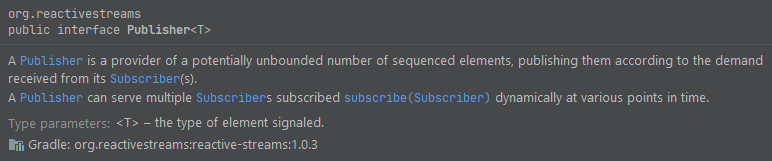
\includegraphics[width=12cm]{img/publisher_api.png}
		};
	\end{tikzpicture}
	
	\begin{tikzpicture}[overlay,remember picture]
		\node[anchor=center,xshift=0pt,yshift=-50pt]
		at (current page.center) {
			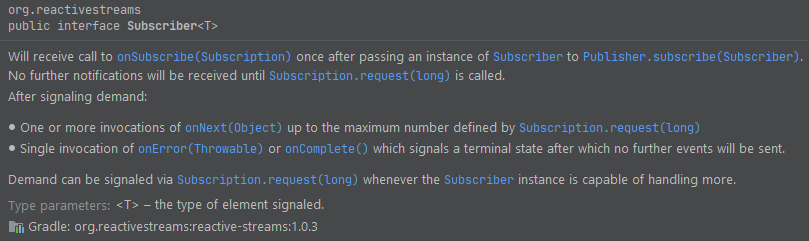
\includegraphics[width=12cm]{img/subscriber_api.png}
		};
	\end{tikzpicture}
\end{frame}

\begin{frame}
	\frametitle{\textit{Publisher} \& \textit{Subscriber} -suite-}
	\begin{tikzpicture}[overlay,remember picture]
		\node[anchor=center,xshift=0pt,yshift=30pt]
		at (current page.center) {
			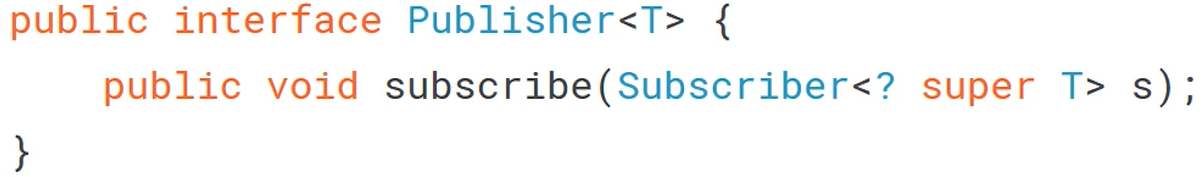
\includegraphics[width=10.2cm]{img/publisher_intf.png}
		};
	\end{tikzpicture}
	
	\begin{tikzpicture}[overlay,remember picture]
		\node[anchor=center,xshift=-17pt,yshift=-50pt]
		at (current page.center) {
			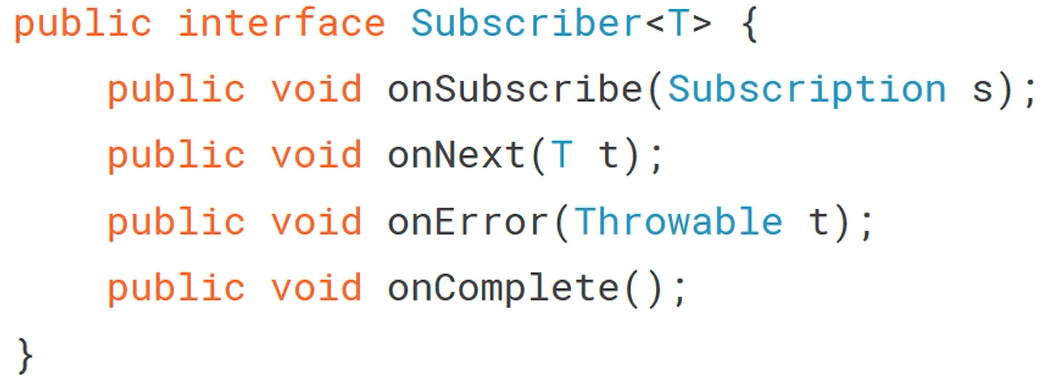
\includegraphics[width=9cm]{img/subscriber_intf.png}
		};
	\end{tikzpicture}
\end{frame}

\begin{frame}
	\frametitle{\textit{Subscription}}
	\begin{tikzpicture}[overlay,remember picture]
		\node[anchor=center,xshift=0pt,yshift=30pt]
		at (current page.center) {
			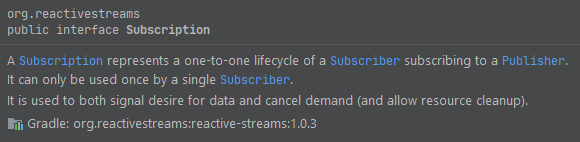
\includegraphics[width=10.2cm]{img/subscription_api.png}
		};
	\end{tikzpicture}
	
	\begin{tikzpicture}[overlay,remember picture]
		\node[anchor=center,xshift=-45pt,yshift=-50pt]
		at (current page.center) {
			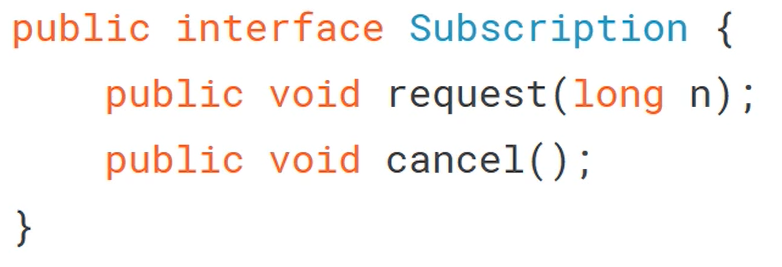
\includegraphics[width=7cm]{img/subscription_intf.png}
		};
	\end{tikzpicture}
	\begin{itemize}
		\vspace{4.5cm}
		\item[] \texttt{request()} permet de mettre en place la \textit{backpressure}
		(demander \texttt{n} éléments que le \textit{subscriber} est capable de traiter)
	\end{itemize}
\end{frame}

\begin{frame}
	\frametitle{Flux de données}
	
	\begin{tikzpicture}[overlay,remember picture]
		\node[anchor=center,xshift=0pt,yshift=0pt]
		at (current page.center) {
			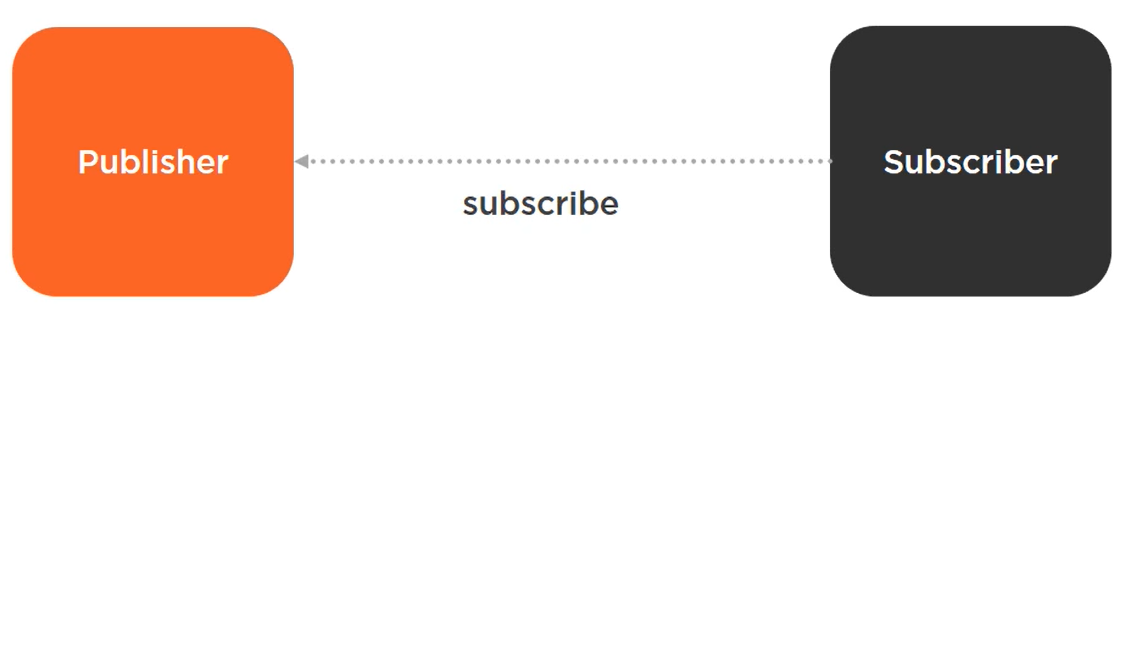
\includegraphics[width=10cm]{img/data_flow_1.png}
		};
	\end{tikzpicture}
	\begin{itemize}
		\vspace{5.5cm}
		\item Le \textit{subscriber} souscrit à un \textit{publisher}
	\end{itemize}
\end{frame}

\begin{frame}

\frametitle{Flux de données}	
	
	\begin{tikzpicture}[overlay,remember picture]
		\node[anchor=center,xshift=0pt,yshift=0pt]
		at (current page.center) {
			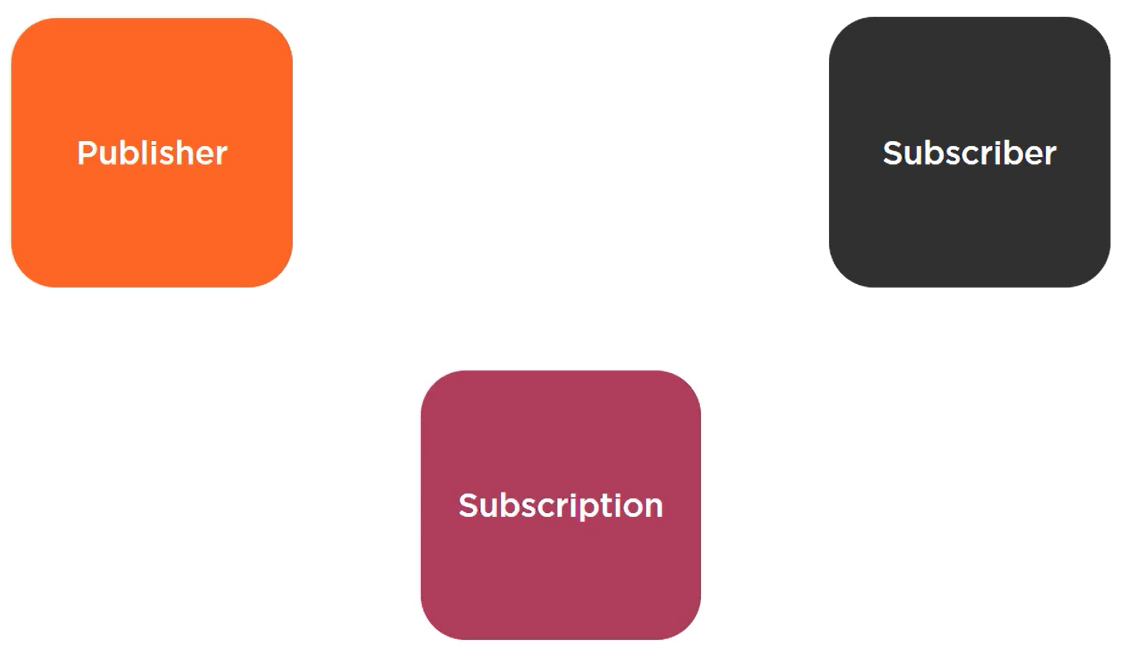
\includegraphics[width=10cm]{img/data_flow_2.png}
		};
	\end{tikzpicture}
	\begin{itemize}
		\vspace{5.5cm}
		\item Un objet \textit{subscription} est créé
	\end{itemize}
\end{frame}

\begin{frame}
	
\frametitle{Flux de données}	

\begin{tikzpicture}[overlay,remember picture]
	\node[anchor=center,xshift=0pt,yshift=0pt]
	at (current page.center) {
		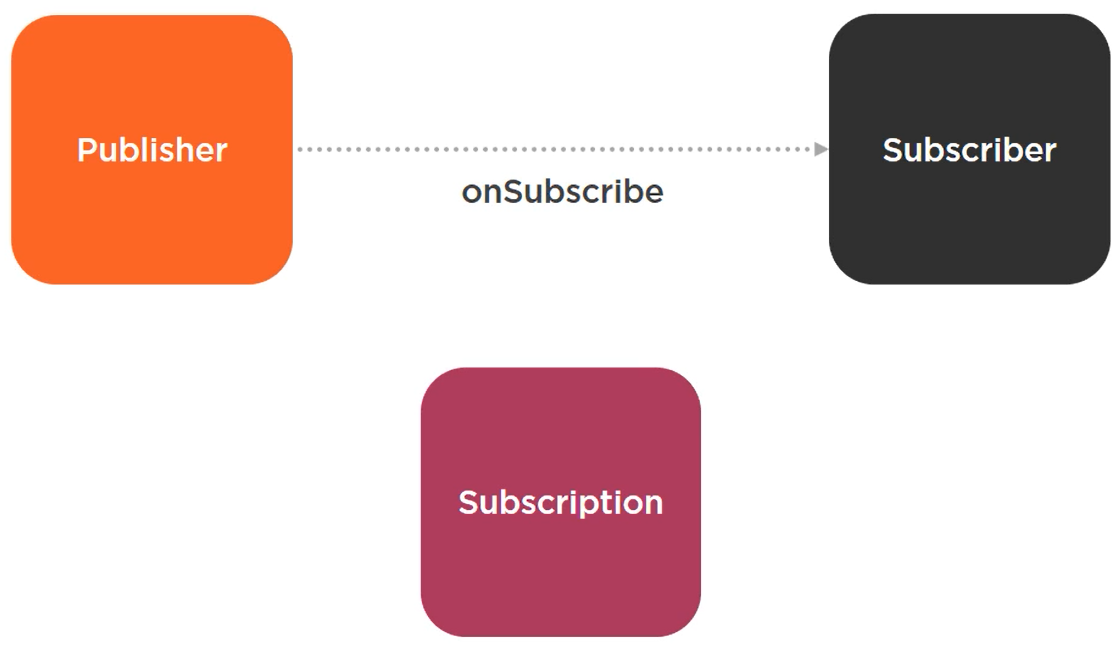
\includegraphics[width=10cm]{img/data_flow_3.png}
	};
\end{tikzpicture}
	\begin{itemize}
		\vspace{5.5cm}
		\item La méthode \textit{onSubscribe()} du \textit{subscriber} est invoquée et l'objet \textit{subscription} est passé en argument
	\end{itemize}
\end{frame}

\begin{frame}
	
	\frametitle{Flux de données}	
	
	\begin{tikzpicture}[overlay,remember picture]
		\node[anchor=center,xshift=0pt,yshift=0pt]
		at (current page.center) {
			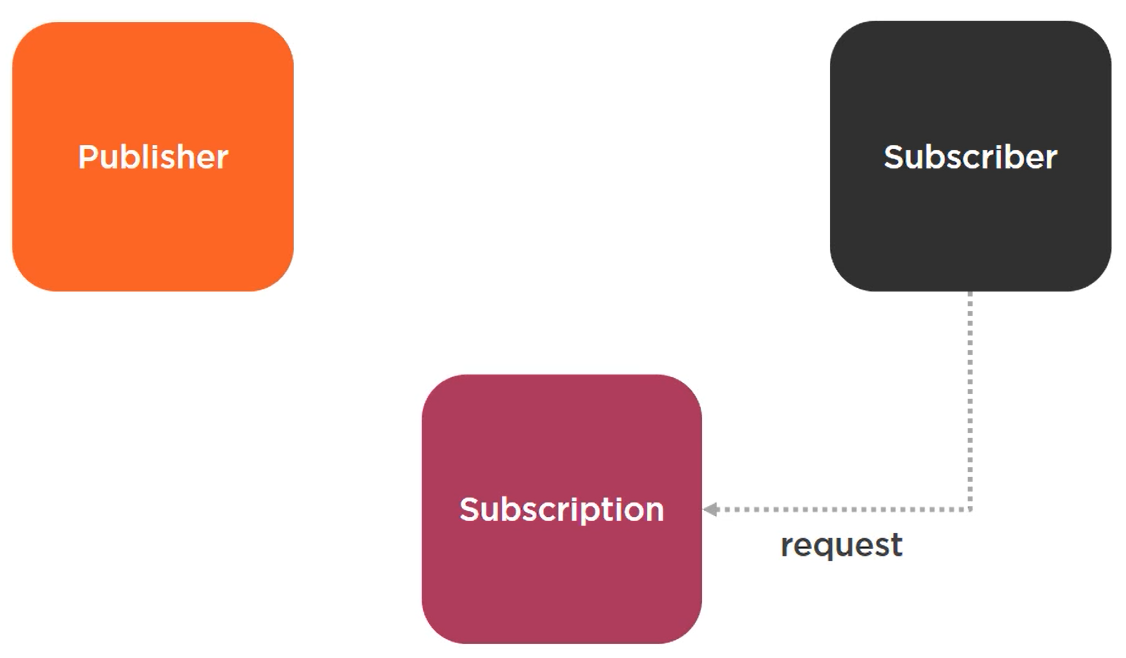
\includegraphics[width=10cm]{img/data_flow_4.png}
		};
	\end{tikzpicture}
	\begin{itemize}
		\vspace{5.5cm}
		\item Le \textit{subscriber} utilise la \textit{subscription} pour indiquer combien de données il est capable de traiter (avec \texttt{request})
	\end{itemize}
\end{frame}

\begin{frame}
	
	\frametitle{Flux de données}	
	
	\begin{tikzpicture}[overlay,remember picture]
		\node[anchor=center,xshift=0pt,yshift=0pt]
		at (current page.center) {
			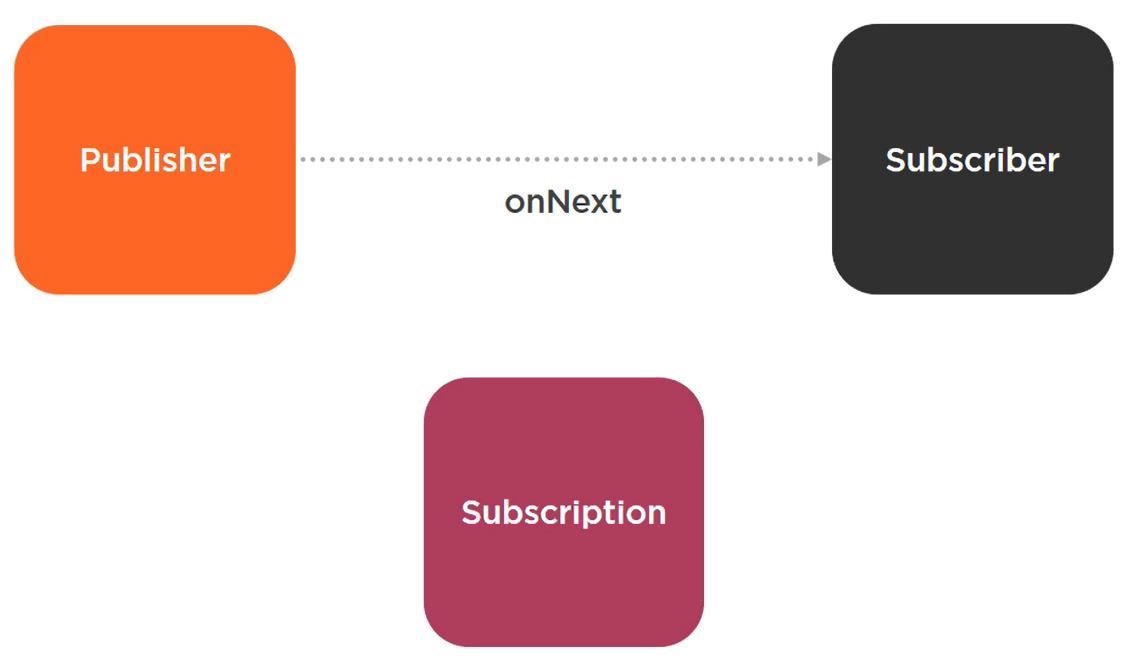
\includegraphics[width=10cm]{img/data_flow_5.png}
		};
	\end{tikzpicture}

\begin{itemize}
	\vspace{5.5cm}
	\item onNext() est invoquée et une donnée est passée en argument
	\item C'est fait plusieurs fois (n fois -- n indiqué dans \textit{request})
\end{itemize}
	
\end{frame}

\begin{frame}	
	\frametitle{Flux de données}	
	\begin{tikzpicture}[overlay,remember picture]
		\node[anchor=center,xshift=0pt,yshift=0pt]
		at (current page.center) {
			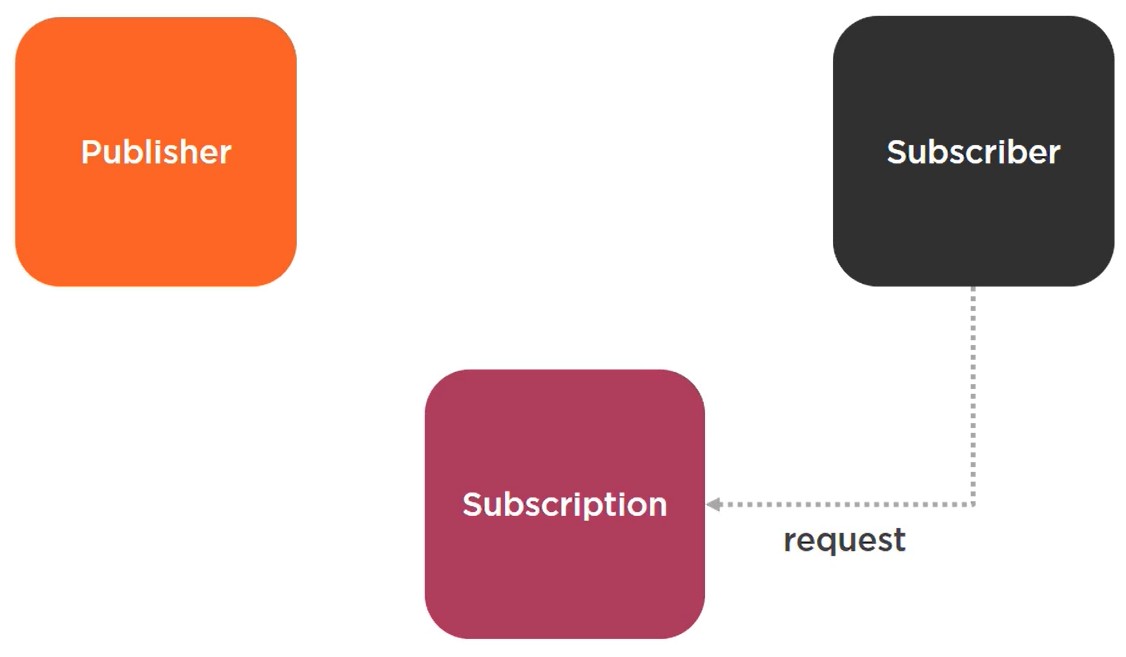
\includegraphics[width=10cm]{img/data_flow_6.png}
		};
	\end{tikzpicture}
	
	\begin{itemize}
		\vspace{5.5cm}
		\item Soit le \textit{subscriber} demande de nouvelles données
	\end{itemize}
\end{frame}

\begin{frame}	
	\frametitle{Flux de données}	
	\begin{tikzpicture}[overlay,remember picture]
		\node[anchor=center,xshift=0pt,yshift=0pt]
		at (current page.center) {
			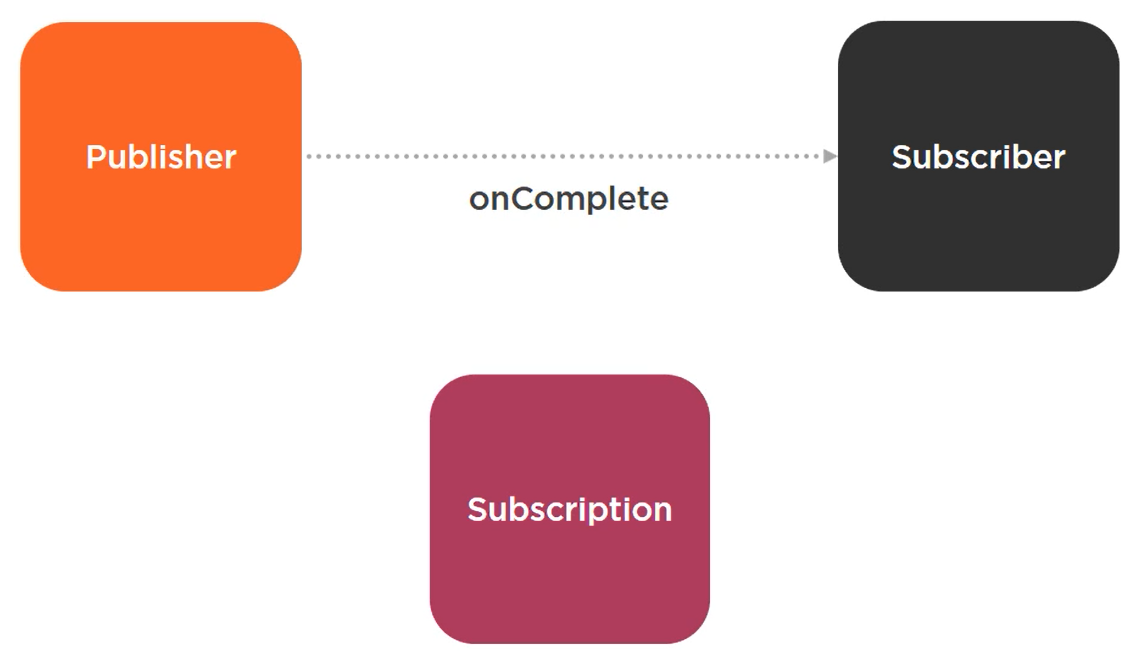
\includegraphics[width=10cm]{img/data_flow_7.png}
		};
	\end{tikzpicture}
	
	\begin{itemize}
		\vspace{5.5cm}
		\item Ou bien, c'est fini, \texttt{onComplete()} de \textit{subscriber} est invoquée et la \textit{subscription} est annulée
	\end{itemize}
\end{frame}

\begin{frame}	
	\frametitle{Flux de données}	
	\begin{tikzpicture}[overlay,remember picture]
		\node[anchor=center,xshift=0pt,yshift=0pt]
		at (current page.center) {
			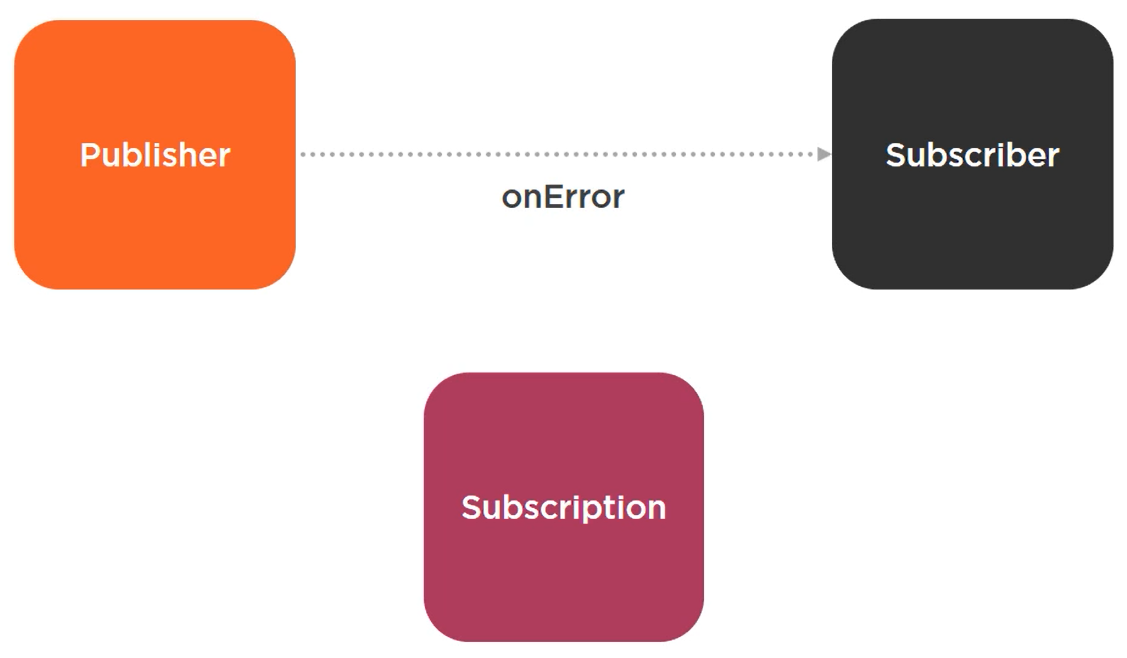
\includegraphics[width=10cm]{img/data_flow_8.png}
		};
	\end{tikzpicture}
	
	\begin{itemize}
		\vspace{5.5cm}
		\item Ou encore, il y a une erreur, \texttt{onError()} de \textit{subscriber} est invoquée et la \textit{subscription} est annulée
	\end{itemize}
\end{frame}

\begin{frame}
	\frametitle{Plusieurs implems de l'API Reactive Streams}
	\begin{itemize}
		\item Reactor
		\item RxJava et RxJava2
		\item CompletableFeature
		\item Java 9+ Flow API
	\end{itemize}
	\textit{(Project) Reactor} est l'implem par défaut (et recommandée) dans Spring Web Flux~:
	\url{https://projectreactor.io/}
\end{frame}

\begin{frame}
	\frametitle{\textit{Publisher}s de \textit{Reactor}}
	\begin{description}
		\item[- \texttt{Mono}] permet de produire 0 ou une donnée
		\begin{itemize}
			\item Mono est l'équivalent \textit{réactif} du type \texttt{Optional} de Java 8+
			\item A utiliser quand on veut retourner dans une méthode 1 objet ou bien void
		\end{itemize}
		\item[- \texttt{Flux}] permet de produire plus d'une donnée
		\begin{itemize}
			\item A utiliser quand on veut retourner une liste
		\end{itemize}
	\end{description}
\end{frame}

\begin{frame}	
	\frametitle{\textit{Marble Diagram} de \texttt{Mono}}	
	\begin{tikzpicture}[overlay,remember picture]
		\node[anchor=center,xshift=0pt,yshift=0pt]
		at (current page.center) {
			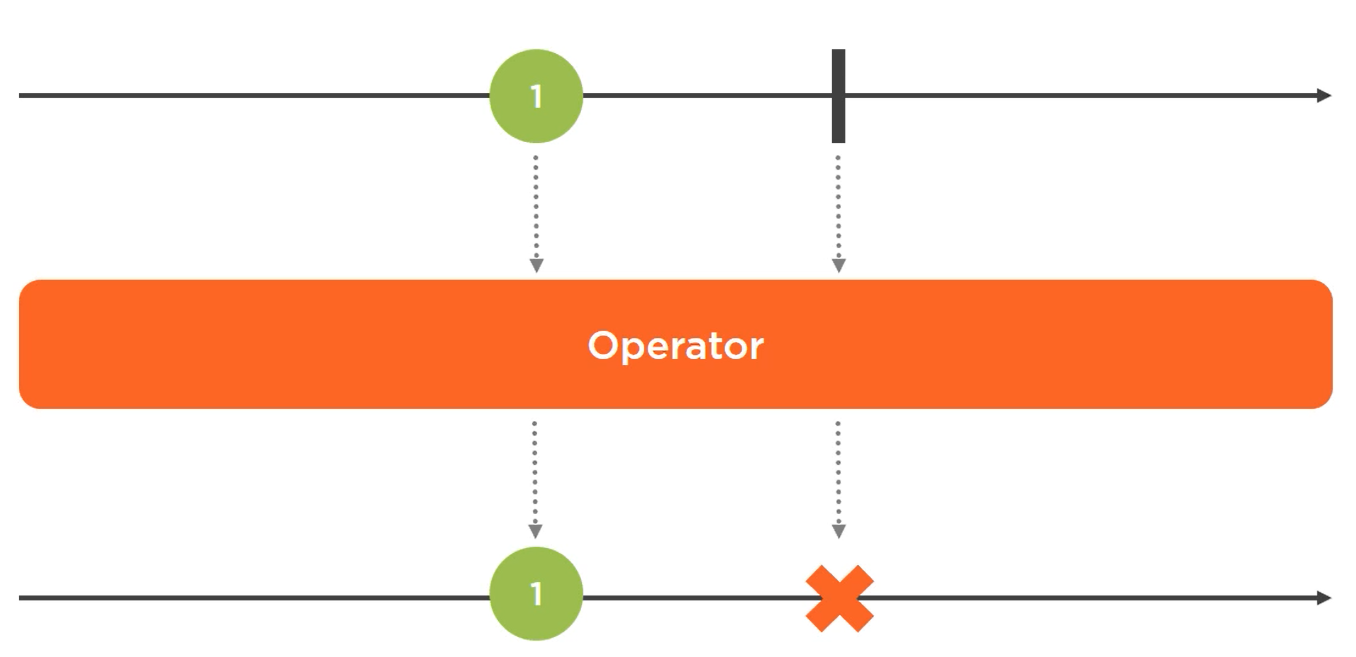
\includegraphics[width=11cm]{img/mono_diag.png}
		};
	\end{tikzpicture}
	
	\begin{itemize}
		\vspace{5.5cm}
		\item Operator permet de transformer ou vérifier la donnée produite
	\end{itemize}
\end{frame}

\begin{frame}	
	\frametitle{\textit{Marble Diagram} de \texttt{Flux}}	
	\begin{tikzpicture}[overlay,remember picture]
		\node[anchor=center,xshift=0pt,yshift=0pt]
		at (current page.center) {
			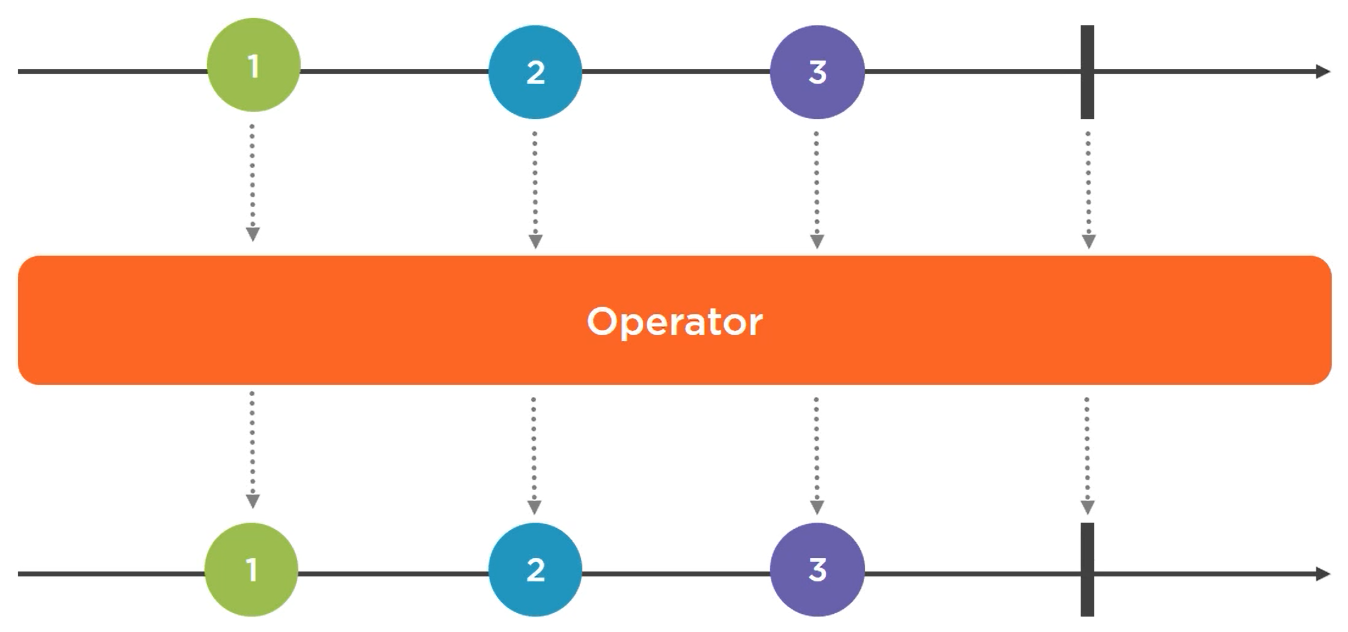
\includegraphics[width=11cm]{img/flux_diag.png}
		};
	\end{tikzpicture}
	
	\begin{itemize}
		\vspace{5.5cm}
		\item La ligne verticale indique le \texttt{onComplete} et la croix le \texttt{onError}
	\end{itemize}
\end{frame}

\begin{frame}[fragile]
	\frametitle{Tester Reactor}	

	\begin{itemize}
		\item Créer un projet Gradle \& Java sur IntelliJ
		\item Ajouter la dépendance suivante~:\\
{\footnotesize
\texttt{implementation 'io.projectreactor:reactor-core:3.4.0'}
}
		\item Dans la classe de test, ajouter une méthode pour tester \texttt{Mono}~:
\end{itemize}		
\begin{lstlisting}
@Test
public void firstMono() {
 Mono.just("A")// Create a Publisher that produces "A" once
 .log()// Log the events	
 .subscribe(s->System.out.println(s));// Create a Subscriber
}
\end{lstlisting}
\begin{itemize}
\item On a créé un \textit{publisher} de type Mono qui produit la chaîne "A"
\item On a créé un \textit{subscriber}, ici un objet \texttt{java.util.function.Consumer} qui correspond à une lambda qui fait un println
	\end{itemize}
\end{frame}

\begin{frame}[fragile]
	\frametitle{Tester Reactor -Mono-}	
	
	\begin{itemize}
		\item Le même exemple avec des écouteurs d'événements~:
	\end{itemize}
\begin{lstlisting}
@Test
public void monoWithDoOn() {
 Mono.just("A") // Publish "A"
 .log() // Log the events
 .doOnSubscribe(subscription 
  -> System.out.println("Subscription : "+subscription))
 .doOnRequest(request 
  -> System.out.println("Request: "+request))
 .doOnSuccess(complete 
  -> System.out.println("Complete: "+complete))
 .subscribe(System.out::println);
}
\end{lstlisting}
	Noter le remplacement de la lambda par une référence de méthode à la dernière ligne
\end{frame}

\begin{frame}[fragile]
	\frametitle{Tester Reactor -Mono-}	
	
	\begin{itemize}
		\item Mono vide~:
\begin{lstlisting}
@Test
public void emptyMono() {
	Mono.empty()
	.log()
	.subscribe(System.out::println);
}
\end{lstlisting}
\item Ici, \texttt{onNext} n'est pas invoquée parce que le Mono ne produit pas une vraie donnée
\item Seule \texttt{onComplete} sera invoquée
\item Mais à quoi sert donc un \texttt{Mono.empty()}~?\\ A simuler un \texttt{return}  dans une méthode \texttt{void} et dire que le process de production du Publisher s'est terminé (mais sans envoi de données)
	\end{itemize}
\end{frame}

\begin{frame}[fragile]
	\frametitle{Tester Reactor -Mono-}	
	
	\begin{itemize}
		\item Mono qui produit une erreur~:
\begin{lstlisting}
@Test
public void monoWithError() {
	Mono.error(new RuntimeException())
	.log()
	.subscribe();
}
\end{lstlisting}
\item Ici, on fait une souscription mais sans indiquer ce qui doit se passer après onNext
\item A l'exécution, vous verrez onError qui affiche la \textit{stack trace} de l'exception
\item Pas de try-catch dans la programmation réactive avec Reactor
\item Possibilité de capture avec onErrorResume ou onErrorReturn
	\end{itemize}
\end{frame}

\begin{frame}[fragile]
	\frametitle{Tester Reactor -Flux-}	
	
	\begin{itemize}
		\item Ajouter une méthode pour tester \texttt{Flux}~:
\begin{lstlisting}
@Test
public void firstFlux() {
	//Flux.just("A","B","C")
	Flux.range(10,5)
	.log()
	.subscribe(System.out::println);
}
\end{lstlisting}
\item Possibilité de faire Flux.fromIterable, .fromArray, .fromStream, fromPublisher, ...

	\end{itemize}
\end{frame}

\begin{frame}[fragile]
	\frametitle{Tester Reactor -Flux-}	
	
	\begin{itemize}
		\item Produire des valeurs avec un intervalle de temps~:\\
		\texttt{Flux.interval(Duration.ofSeconds(1))}\\
		\texttt{Duration} est issue de \texttt{java.time}
\begin{lstlisting}
@Test
public void firstFlux() {
 Flux.interval(Duration.ofSeconds(1))
 .log()
 .subscribe(System.out::println);
 Thread.sleep(5000);
}
\end{lstlisting}
	\item \texttt{interval} démarre dans un nouveau thread la production d'entier à partir de 0 toutes les 1 seconde
	\item On met le \texttt{Thread.sleep} pour ne pas avoir le test qui se termine (et donc le thread créé par interval tué) avant la production des données
	\end{itemize}
\end{frame}

\begin{frame}[fragile]
	\frametitle{Tester Reactor -Flux-}	
	
	\begin{itemize}
		\item Dans l'exemple, onComplete n'est pas invoquée parce que le thread a été tué à la fin de l'exécution du test
		\item Dans une application Web, on a des processus/threads qui s'exécutent en continu
		\item On peut donc avoir une production de valeurs en continu
		\item Pour annuler la production de données au delà d'un certain nombre (de données), on peut utiliser l'opérateur \texttt{take}~:
\begin{lstlisting}
Flux.interval(Duration.ofSeconds(1))
.log()
.take(5) // Annule la souscription apres 5 donnees
.subscribe(System.out::println); Thread.sleep(8000);
\end{lstlisting}
onComplete n'est pas invoquée (ce n 'est pas un mécanisme de \textit{backpressure}). C'est plutôt un cancel (lire la doc de \texttt{take} sur IntelliJ). 
	\end{itemize}
\end{frame}

\begin{frame}[fragile]
	\frametitle{Tester Reactor -Flux-}	
	
	\begin{itemize}
		\item Pour appliquer une \textit{backpressure}, utiliser l'opérateur limitRate~:
\begin{lstlisting}
Flux.range(1,8)
.log()
.limitRate(3)
.subscribe();
\end{lstlisting}
		\item Plus de détails~:
		{\footnotesize \url{https://projectreactor.io/docs/core/release/reference/}}
	\end{itemize}
\end{frame}

\begin{frame}[fragile]
	\frametitle{\textit{Backpressure} avec un subscriber personnalisé}	

\begin{lstlisting}
Flux.range(1, 10)
.log().subscribe(new BaseSubscriber<Integer>() {
 int elementsToProcess = 3; int counter = 0;
 @Override
 protected void hookOnSubscribe(Subscription subs) {
  System.out.println("Subscribed");
  subs.request(elementsToProcess);
 }
 @Override
 protected void hookOnNext(Integer value) {
  counter++;
  if(counter == elementsToProcess) {
   counter = 0;
   Random r = new Random();
   elementsToProcess = r.ints(3,5).findFirst().getAsInt();
   request(elementsToProcess);
  } }
});
\end{lstlisting}
\end{frame}

\begin{frame}
	\frametitle{Quelques opérateurs}
	\begin{enumerate}
		\item map
		\item flatMap
		\item concat et merge
		\item zip
	\end{enumerate}
\end{frame}

\begin{frame}[fragile]
	\frametitle{Opérateur \texttt{map}}
	\begin{itemize}
		\item Similaire à map vue dans l'API Stream (en IG4). Applique une fonction synchrone à chaque donnée du Flux
\begin{lstlisting}
@Test
public void fluxWithMap() {
	Flux.range(1,5)
	.map(i->i*5)
	.subscribe(System.out::println);
}
\end{lstlisting}
\item Survoler le nom de la méthode map sur IntelliJ pour voir sa documentation
	\end{itemize}
\end{frame}

\begin{frame}[fragile]
	\frametitle{Opérateur \texttt{flatMap}}
	\begin{itemize}
		\item Version réactive de map. Doit donc retrouner un Mono ou un Flux~:
\begin{lstlisting}
@Test
public void fluxWithFlatMap() {
	Flux.range(1,5)
	.flatMap(i->Flux.range(i*5,10))
	.subscribe(System.out::println);
}
\end{lstlisting}
		\item Chaque donnée est transformée en un publisher qui exploite la donnée
		\item Survoler le nom de la méthode flatMap sur IntelliJ pour voir son fonctionnement avec le Marble Diagram
	\end{itemize}
\end{frame}

\begin{frame}[fragile]
	\frametitle{Opérateur \texttt{flatMapMany}}
	\begin{itemize}
		\item Transforme un Mono en un Flux
\begin{lstlisting}
@Test
public void fluxWithFlatMapMany() {
	Mono.just(3)
	.flatMapMany(i->Flux.range(1,i))
	.subscribe(System.out::println);
}
\end{lstlisting}
		\item Crée un Flux à partir d'un Mono en exploitant la donnée produite par le Mono
	\end{itemize}
\end{frame}

\begin{frame}[fragile]
	\frametitle{Opérateurs \texttt{concat} et \texttt{merge}}
	\begin{itemize}
		\item \texttt{concat} concatène les données produites par des publishers
\begin{lstlisting}
@Test
public void fluxWithConcat() throws InterruptedException {
	Flux<Integer> oneToFive = Flux.range(1,5)
	.delayElements(Duration.ofMillis(200));
	Flux<Integer> sixToTen = Flux.range(6,5)
	.delayElements(Duration.ofMillis(400));
	Flux.concat(oneToFive,sixToTen)
	.subscribe(System.out::println);
	Thread.sleep(5000);
}
\end{lstlisting}
\item Noter l'utilisation de l'opérateur \texttt{delayElements} poure retarder la production de chaque donnée (élément)
\item Un autre opérateur \texttt{merge} mélange les données des deux publishers
(le tester pour voir la différence)
	\end{itemize}
\end{frame}

\begin{frame}[fragile]
	\frametitle{Opérateur \texttt{zip}}
	\begin{itemize}
		\item Transforme les données des publishers et produit un nouveau publisher qui produit les données transformées
\begin{lstlisting}
@Test
public void fluxWithZip() {
	Flux<Integer> oneToFive = Flux.range(1,5);
	Flux<Integer> sixToTen = Flux.range(6,5);
	Flux.zip(oneToFive,sixToTen,
	  (item1,item2)->item1+"-"+item2)
	.subscribe(System.out::println);
}
\end{lstlisting}
Tester pour voir
	\end{itemize}
Sur le site de \textit{Project Reactor}, vous avez une bonne documentation, et notamment dans l'annexe A, on vous indique quel opérateur utiliser dans vos programmes
\end{frame}


\section{Développer une API REST réactive avec des contrôleurs annotés}

\begin{frame}		
	\frametitle{Spring Web Flux vs Spring MVC}
	\begin{tikzpicture}[overlay,remember picture]
		\node[anchor=center,xshift=0pt,yshift=-30pt]
		at (current page.center) {
			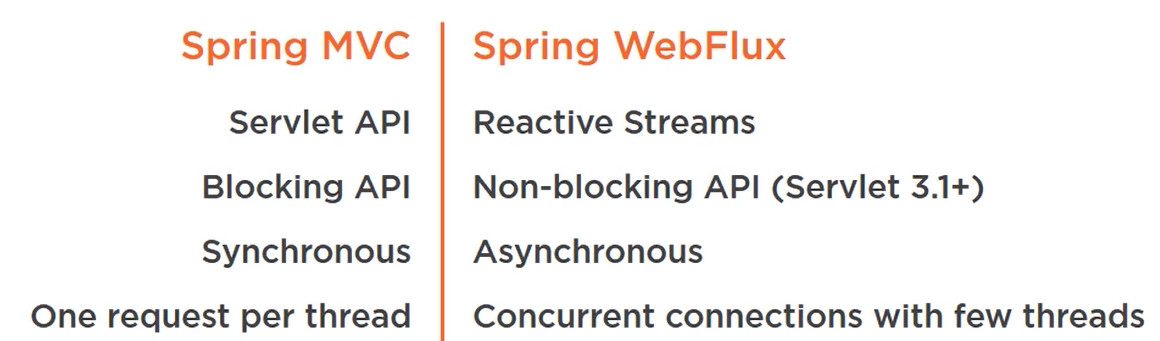
\includegraphics[width=11cm]{img/web_flux_vs_mvc.png}
		};
	\end{tikzpicture}
	
	\begin{itemize}
		\item Spring Web Flux est une alternative à Spring MVC, qui permet d'écrire des app Web réactives
		\vspace{5cm}
	\end{itemize}
\end{frame}

\begin{frame}		
	\frametitle{Spring Web Flux vs Spring MVC}	
	\begin{tikzpicture}[overlay,remember picture]
		\node[anchor=center,xshift=0pt,yshift=0pt]
		at (current page.center) {
			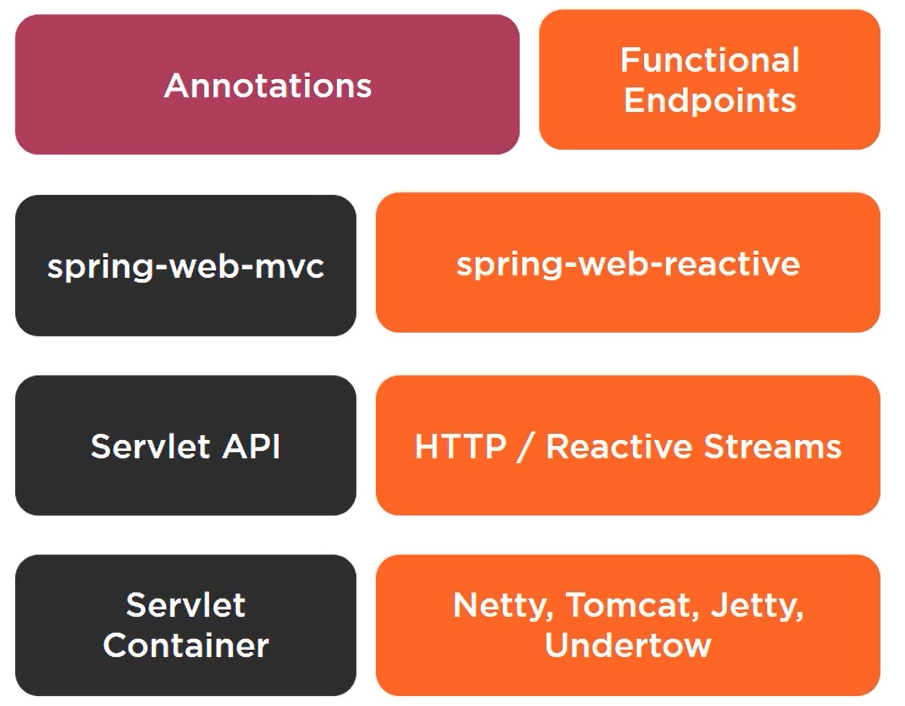
\includegraphics[width=8cm]{img/servlet_vs_reactive_streams.png}
		};
	\end{tikzpicture}
\begin{itemize}
	\vspace{5.5cm}
	\item[] Dans cette section, on voit comment utiliser les annotations pour écrire une API REST réactive
\end{itemize}
\end{frame}

\begin{frame}		
	\frametitle{\textit{Reactive} partout}	
	\begin{tikzpicture}[overlay,remember picture]
		\node[anchor=center,xshift=0pt,yshift=-10pt]
		at (current page.center) {
			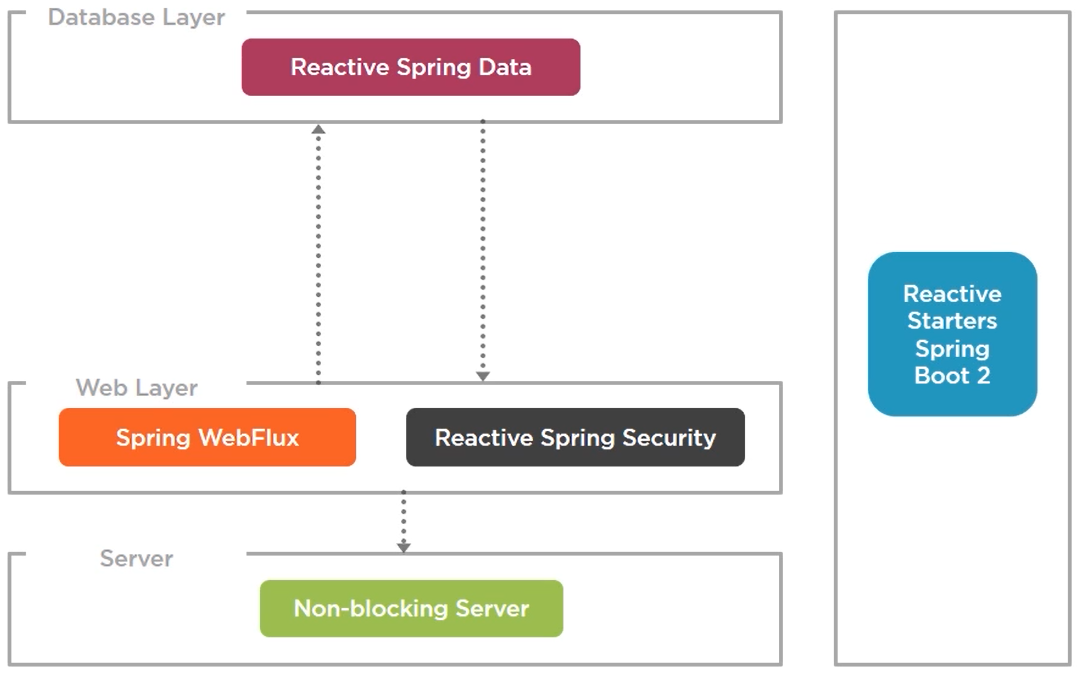
\includegraphics[width=11cm]{img/reactive_partout.png}
		};
	\end{tikzpicture}
\end{frame}

\begin{frame}[fragile]
	\frametitle{Exemple que l'on va écrire dans cette partie}
	\begin{itemize}
		\item Un contrôleur annoté WebFlux pour envoyer des informations (des nouvelles) Covid aux utilisateurs
		\begin{itemize}
			\item Les annotations WebFlux et Web MVC sont les mêmes (@Controller (contrôleur de vues), @RestController (contrôleur d'API Rest -- données JSON par ex), @RequestMapping, @GetMapping, ...)
		\end{itemize}
		\item Nous allons utiliser une base de données NoSQL (à documents) MongoDB pour stocker les infos COVID
		\item Nous allons utiliser \textit{Server Sent Events} (cours IG3-FAR sur les websockets) comme moyen de faire du Server Push
	\end{itemize}
\end{frame}

\begin{frame}[fragile]
	\frametitle{Requêtes et réponses HTTP réactives}
	\begin{itemize}
		\item Spring Web Flux introduit des classes particulières pour représenter les requêtes et réponses HTTP réactives~: \texttt{ServerHttpRequest} et \texttt{ServerHttpResponse}
		\item Les méthodes des contrôleurs peuvent utiliser les types habituels dans Spring MVC (String, ResponseEntity, ...) ou bien Mono et Flux comme type de retour pour retourner des données (voir les exemples qui vont suivre)
	\end{itemize}
\end{frame}

\begin{frame}[fragile]
	\frametitle{Initialiser un nouveau projet}
	\begin{itemize}
		\item Aller sur le site Spring Initializr~:
		\url{https://start.spring.io/}
		\item Configurer un nouveau projet (Gradle \& Java) en ajoutant les dépendances suivantes~:
		\begin{itemize}
			\item Reactive Web
			\item Reactive MongoDB (qui vient avec le driver \textit{reactive} de MongoDB)
			\item Embedded MongoDB (serveur de BdD)
		\end{itemize}
	\end{itemize}
\end{frame}

\begin{frame}[fragile]
	\frametitle{Initialiser un nouveau projet -suite-}
	\begin{itemize}
	\item Embedded MongoDB est considéré comme un serveur à utiliser pour les tests. Si vous avez dans votre script de build \texttt{testImplementation} devant cette dépendance, changez la en \texttt{implementation}
	\item Il faudrait avoir les dépendances suivantes~:
	\end{itemize}
\begin{lstlisting}
dependencies {
 implementation 'org.springframework.boot:spring-boot-starter-webflux'	
 implementation 'org.springframework.boot:spring-boot-starter-data-mongodb-reactive'
 implementation 'de.flapdoodle.embed:de.flapdoodle.embed.mongo'
 testImplementation 'org.springframework.boot:spring-boot-starter-test'
 testImplementation 'io.projectreactor:reactor-test'
}
\end{lstlisting}
\end{frame}

\begin{frame}[fragile]
	\frametitle{Le modèle dans l'application}
	\begin{itemize}
		\item Créer un package model et une classe \texttt{CovidInfo} dans ce package
		\item Dans cette classe, ajouter~:
		\begin{itemize}
			\item une annotation @Document (pour que nos entités correspondent à des documents dans MongoDB)
			\item un attribut annoté @Id de type String et nommé id
			\item les attributs suivants~:
\begin{lstlisting}
private String title; // titre de l'info Covid
private String content; // contenu de l'info
private LocalDateTime publicationDate;
\end{lstlisting}
\item Un constructeur sans paramètre et 1, avec tous les attributs
		\end{itemize}
	\item Générer avec IntelliJ les getters, setters, equals, hashCode et toString
	\end{itemize}
\end{frame}

\begin{frame}[fragile]
	\frametitle{Le \textit{repository}}
	\begin{itemize}
		\item Créer un package repository et une interface \texttt{CovidInfoRespository}~:
	\end{itemize}
\begin{lstlisting}
import org.springframework.data.mongodb.repository.ReactiveMongoRepository;
import poly.mtp.infoapi.model.CovidInfo;
import reactor.core.publisher.Flux;
import java.time.LocalDateTime;
public interface CovidInfoRepository
 extends ReactiveMongoRepository<CovidInfo,String> {
 Flux<CovidInfo> findByTitleOrderByPublicationDate(String title);
 Flux<CovidInfo> findByPublicationDateOrderByTitle(Date publicationDate);
}
\end{lstlisting}
Notez les méthodes ajoutées à l'interface pour faire des find avec autre chose que l'id (ces méthodes doivent respecter des conventions de nommage Spring Data)
\end{frame}

\begin{frame}[fragile]
	\frametitle{Mettre en place la base de données}
	\begin{itemize}
		\item Dans la classe annotée \texttt{@SpringBootApplication}, ajouter l'annotation 
		@EnableMongoRepositories
		\item Y ajouter la méthode suivante pour initialiser la BdD~:
	\end{itemize}
\begin{lstlisting}
@Bean
CommandLineRunner init(CovidInfoRepository repository) {
 return args -> {
  Flux<CovidInfo> covidInfoFlux = Flux.just(
  new CovidInfo(null, "Point de situation",
   "Nouveaux cas confirmes ...", LocalDateTime.now()),
  new CovidInfo(null, "Informations sur les mesures 
   nationales", "Le 22.11.2021 ..",LocalDateTime.now()))
  .flatMap(repository::save);
  // Just to check if data has been inserted
  covidInfoFlux.thenMany(repository.findAll())
  .subscribe(System.out::println);
 };
}
\end{lstlisting}
	
\end{frame}

\begin{frame}[fragile]
	\frametitle{Tester votre application}
	\begin{itemize}
		\item Faire un bootRun pour démarrer l'application
		\item Si jamais vous avez une erreur lors du téléchargement de MongoDB (téléchargement trop lent, connexion instable, ...), télécharger à la main le ZIP du site \url{http://downloads.mongodb.org} et l'installer dans le dossier \texttt{.embedmongo} de votre \texttt{user.home}
% Pour Windows: \url{http://downloads.mongodb.org/win32/mongodb-win32-x86_64-3.5.5.zip}
		\item Ceci permet à Gradle d'aller le chercher dans ce dossier plutôt que de le télécharger
		\item Il faut que vous soyez capables de voir les données, insérées dans la base, affichées dans la console par le println du subscriber ci-dessus
	\end{itemize}
\end{frame}

\begin{frame}[fragile]
	\frametitle{Le contrôleur}
	\begin{itemize}
		\item Ajouter un package controller et une classe \texttt{CovidInfoController} annotée de la façon suivante~:
\begin{lstlisting}
@RestController
@RequestMapping("/infos")
\end{lstlisting}
	\item Ajouter un attribut auto-injecté pour avoir accès au repository~:
\begin{lstlisting}
@Autowired
CovidInfoRepository repository;
\end{lstlisting}
\item Ajouter une méthode Get (pour obtenir toutes les infos)~:
\begin{lstlisting}
@GetMapping
public Flux<CovidInfo> getAllInfos() {
	return repository.findAll();
}
\end{lstlisting}
Noter le type de retour Flux. Pas de \textit{subscriber} ici, Spring le fera automatiquement
	\end{itemize}
\end{frame}

\begin{frame}[fragile]
	\frametitle{Autres méthodes du contrôleur}
	\begin{itemize}
		\item Obtenir une info avec son ID~:
\begin{lstlisting}
@GetMapping("{id}")
public Mono<ResponseEntity<CovidInfo>> getInfo(@PathVariable String id) {
	return repository.findById(id).map(covidInfo -> ResponseEntity.ok(covidInfo))
	.defaultIfEmpty(ResponseEntity.notFound().build());
}
\end{lstlisting}
\item Noter le type de retour Mono (une réponse unique)
\item Retourner le résultat de findById provoque l'envoi d'un empty (réponse 200) si jamais l'info avec l'Id reçu n'existe pas
\item C'est pour cela que cette méthode utilise map pour retourner une réponse 200 avec l'info Covid ou bien retourne une réponse 404 (type de retour : \texttt{Mono<ResponseEntity<CovidInfo>~>})
	\end{itemize}
\end{frame}

\begin{frame}[fragile]
	\frametitle{Autres méthodes du contrôleur -suite-}
	\begin{itemize}
		\item Méthode POST simplifiée~:
\begin{lstlisting}
@PostMapping
@ResponseStatus(HttpStatus.CREATED)
public Mono<CovidInfo> saveCovidInfo(@RequestBody CovidInfo covidInfo) {
	return repository.save(covidInfo);
}
\end{lstlisting}
\item Méthode deleteAll~:
\begin{lstlisting}
@DeleteMapping
public Mono<Void> deleteAllProducts() {
	return repository.deleteAll();
}
\end{lstlisting}
	\end{itemize}
\end{frame}

\begin{frame}[fragile]
	\frametitle{Autres méthodes du contrôleur -suite-}
	\begin{itemize}
		\item Méthode delete une info~:
\begin{lstlisting}
@DeleteMapping("{id}")
public Mono<ResponseEntity<Void>> deleteInfo(@PathVariable("id") String id) {
 return repository.findById(id)
  .flatMap(existingCovidInfo ->
   repository.delete(existingCovidInfo)
   .then(Mono.just(ResponseEntity.ok().<Void>build()))
  )
  .defaultIfEmpty(ResponseEntity.notFound().build());
}
\end{lstlisting}
Noter l'utilisation de flatMap pour produire, à partir du premier Mono qui a fait une recherche de l'info, un deuxième Mono qui, après avoir supprimé l'info, construit une réponse Void
	\end{itemize}
\end{frame}

\begin{frame}[fragile]
	\frametitle{Autres méthodes du contrôleur -suite-}
	\begin{itemize}
		\item Méthode de mise à jour d'une info Covid~:
\begin{lstlisting}
@PutMapping("{id}")
public Mono<ResponseEntity<CovidInfo>> updateInfo(@PathVariable("id") String id,
CovidInfo covidInfo) {
 return repository.findById(id)
 .flatMap(existingCovidInfo -> {
  existingCovidInfo.setContent(covidInfo.getContent());
  existingCovidInfo.setTitle(covidInfo.getTitle());
  existingCovidInfo.setPublicationDate(covidInfo.getPublicationDate());
  return repository.save(existingCovidInfo);
  })
  .map(updatedInfo -> ResponseEntity.ok(updatedInfo))
  .defaultIfEmpty(ResponseEntity.notFound().build());
}
\end{lstlisting}
Noter les flatMap puis map pour construire la réponse
	\end{itemize}
\end{frame}

\begin{frame}
	\frametitle{Tester l'application}
	\begin{itemize}
		\item Démarrer votre application
		\item Tester le contrôleur avec des requêtes vers les différentes routes sur votre navigateur et sur Postman ou Curl
		
	\end{itemize}
\end{frame}

\begin{frame}[fragile]
	\frametitle{Méthode dans le contrôleur pour \textit{SSE~: Server Sent Events}}
	\begin{itemize}
		\item Nous allons ajouter une méthode dans le contrôleur pour retourner les infos, mais dans une réponse HTTP avec les \textit{SSE~: Server Sent Events} pour que le serveur effectue des push (quand il y a des nouvelles infos COVID) sans que le client n'envoie une requête
		\item Nous allons d'abord ajouter dans le modèle une classe \texttt{CovidInfoEvent} avec les deux attributs suivants~:
\begin{lstlisting}
private long eventId;
private String eventType;
\end{lstlisting}
Y ajouter deux constructeurs (sans param et avec des param pour initialiser tous les attributs), des getters/setters, equals, hashCode et toString
	\end{itemize}
\end{frame}

\begin{frame}[fragile]
	\frametitle{Méthode dans le contrôleur pour \textit{SSE~: Server Sent Events}}
	\begin{itemize}
		\item Ajouter la méthode suivante au contrôleur~:
\begin{lstlisting}
@GetMapping(value = "/events",produces = MediaType.TEXT_EVENT_STREAM_VALUE)
public Flux<CovidInfoEvent> getInfoEvents() {
 return Flux.interval(Duration.ofSeconds(1))
  .map(val->
  new CovidInfoEvent(val,"Covid Info Event"));
}
\end{lstlisting}
Tester cette route depuis votre navigateur (Chrome supporte les SSE)
	\end{itemize}
\end{frame}

\begin{frame}[fragile]
	\frametitle{Client HTML à cette route}
	\begin{itemize}
		\item Créer un dossier \texttt{public} sous le dossier \texttt{resources}
		\item Ajouter un fichier \texttt{index.html} dans le dossier \texttt{resources/public}
		\item Y ajouter le code suivant~: à tester
\begin{lstlisting}[language=Html]
<h3>Here are the infos received from Covid Server</h3>
<ul></ul>
<script>
if(!!window.EventSource) {
 let eventSource = new EventSource("infos/events/");
 let eventList = document.querySelector("ul");
 eventSource.onmessage = function(e) {
  let newElement = document.createElement("li");
  newElement.textContent = "Event: "+e.data;
  eventList.append(newElement);
 } }
else { alert("Your browser does not support SSE"); }
</script>	
\end{lstlisting}
	\end{itemize}
\end{frame}

\section{Développer une API REST réactive avec des \textit{endpoints} fonctionnels}

\begin{frame}[fragile]
	\frametitle{\textit{Endpoints} fonctionnels}
	\begin{itemize}
		\item C'est une alternative aux contrôleurs annotés
		\item S'appuyer sur le style de programmation fonctionnelle
		\item Il s'agit d'écrire des fonctions qui ne sont pas annotées comme ce que l'on a vu dans la section précédente, mais plutôt retourner des lambdas
		\item Il s'agit d'écrire : 1)~des fonctions \textit{Handler} et 2)une fonction \textit{Router}
	\end{itemize}
\end{frame}

\begin{frame}[fragile]
	\frametitle{Fonctions \textit{Handler}}
	\begin{itemize}
		\item N'importe quelle méthode qui reçoit un objet \texttt{ServerRequest} ({\scriptsize \texttt{org.springframework.web.reactive.function.server.ServerRequest}}) comme paramètre et qui retourne un objet \texttt{Mono<ServerResponse>}
		\item Les deux sont des objets gérés de façon asynchrone
		\item Exemple : fonction handler pour des requêtes Get (toutes les infos Covid)~:
\begin{lstlisting}
public Mono<ServerResponse> getAllInfos(ServerRequest request) {
	Flux<CovidInfo> infos = repository.findAll();
	return ServerResponse.ok()
	.contentType(MediaType.APPLICATION_JSON)
	.body(infos,CovidInfo.class);
}
\end{lstlisting}
	\end{itemize}
\end{frame}

\begin{frame}[fragile]
	\frametitle{Fonction \textit{Router}}
	\begin{itemize}
		\item Cette fonction traite les requêtes Http en premier
		\item C'est une méthode qui prend en paramètre un objet de type \texttt{ServerRequest} et qui retourne un objet \texttt{RouterFunction<ServerResponse>}~:
\begin{lstlisting}
RouterFunction<ServerResponse> routes(CovidInfoHandler handler) {
	// ...
}
\end{lstlisting}
	\texttt{CovidInfoHandler} est la classe qui contient les fonction handlers
	\end{itemize}
\end{frame}

\begin{frame}[fragile]
	\frametitle{Fonction \textit{Router} -suite-}
	On définit dans la fonction précédente les routes~:	
\begin{lstlisting}
RouterFunctions.route(RequestPredicate,HandlerFunction)
\end{lstlisting}
	\begin{itemize}
	\item \texttt{RequestPredicate} est une interface fonctionnelle qui représente une fonction qui permet de tester si la requête match avec un certain chemin (\textit{path}) ou une méthode HTTP
	\item \texttt{HandlerFunction} est une référence vers une fonction handler ou une lambda dans laquelle on invoque une méthode handler
	\item Il existe plusieurs méthodes statiques qu'on peut utiliser comme \texttt{RequestPredicate}, comme \texttt{accept(MediaType...)}, \texttt{method(HttpMethod)}, \texttt{path(String)}, ... de la classe~:
	{\scriptsize \texttt{org.springframework.web.reactive.function.server.RequestPredicates} }
	\end{itemize}
\begin{lstlisting}
RouterFunctions.route(GET("/infos").and(accept(APPLICATION_JSON)), handler::getAllInfos)
\end{lstlisting}
\end{frame}

\begin{frame}[fragile]
	\frametitle{Projet à mettre en place}
	\begin{itemize}
		\item Générer un projet sur Spring Initializr équivalent au projet précédent (mêmes dépendances)
		\item Remplacer testImplementation par implementation pour Embedded MongoDB
		\item Créer un package model et y mettre la classe CovidInfo (la même qu'avant)
		\item Ajouter dans le même package la classe CovidInfoEvent (la même qu'avant)
		\item Créer un package repository et y mettre l'interface CovidInfoRepository (la même qu'avant)
		\item Ajouter dans la classe qui contient main la même méthode d'initialisation de la Bdd (la méthode init)
	\end{itemize}
\end{frame}

\begin{frame}[fragile]
	\frametitle{Projet à mettre en place}
	\begin{itemize}
		\item Créer un package handler
		\item Dans ce package, créer la classe CovidInfoHandler et l'annoter \texttt{@Component}
		\item Ajouter dans cette classe un attribut de type CovidInfoRespository
		\item Ajouter un constructeur avec un paramètre de type CovidInfoRespository qu'il faudra utiliser pour initialiser l'attribut. Spring injectera automatiquement le paramètre du constructeur quand il créera le bean CovidInfoHandler
		\item On va maintenant définir les fonctions handler
	\end{itemize}
\end{frame}

\begin{frame}[fragile]
	\frametitle{Fonctions Handler Get}
\begin{lstlisting}
public Mono<ServerResponse> getAllInfos(
       ServerRequest request) {
	Flux<CovidInfo> infos = repository.findAll();
	return ServerResponse.ok()
	.contentType(MediaType.APPLICATION_JSON)
	.body(infos,CovidInfo.class);
}
\end{lstlisting}
Méthode qui invoque findAll() du repository et construit un Mono de ServerResponse avec dans son body les objets CovidInfo
\end{frame}

\begin{frame}[fragile]
\frametitle{Fonctions Handler Get -suite-}
\begin{lstlisting}
public Mono<ServerResponse> getCovidInfo(
       ServerRequest request) {
	String id = request.pathVariable("id");
	Mono<CovidInfo> infoMono = repository.findById(id);
	Mono<ServerResponse> notFound = ServerResponse.notFound().build();	
	return infoMono.flatMap(
	covidInfo -> ServerResponse.ok()
	.contentType(MediaType.APPLICATION_JSON)
	.body(covidInfo,CovidInfo.class))
	.switchIfEmpty(notFound); // un if-else reactive
}
\end{lstlisting}
	\begin{itemize}
		\item Cette méthode récupère l'id de l'objet request reçu en paramètre, fait un findById, prévoit une réponse NotFound et enfin construit le Mono de ServerResponse avec soit la réponse avec dans son body l'info covid, soit la réponse 404
	\end{itemize}
\end{frame}

\begin{frame}[fragile]
	\frametitle{Fonction Handler Post}
\begin{lstlisting}
public Mono<ServerResponse> saveCovidInfo(ServerRequest request) {
	Mono<CovidInfo> infoMono = request.bodyToMono(CovidInfo.class);
	return infoMono.flatMap(
	covidInfo -> ServerResponse.status(HttpStatus.CREATED)
	.contentType(MediaType.APPLICATION_JSON)
	.body(repository.save(covidInfo),CovidInfo.class));
}
\end{lstlisting}	
	\begin{itemize}
		\item Même schéma, avec une réponse avec le code 201 (CREATED)
	\end{itemize}
\end{frame}

\begin{frame}[fragile]
	\frametitle{Fonction Handler Put}
\begin{lstlisting}[basicstyle=\tiny]
public Mono<ServerResponse> updateCovidInfo(ServerRequest request) {
 String id = request.pathVariable("id");
 Mono<CovidInfo> existingInfoMono=repository.findById(id); 
 Mono<CovidInfo> infoMono=request.bodyToMono(CovidInfo.class);	 
 Mono<ServerResponse> notFound=ServerResponse.notFound().build();
 
 return infoMono.zipWith(existingInfoMono,
  (CovidInfo covidInfo, CovidInfo existingCovidInfo) ->
   new CovidInfo(existingCovidInfo.getId(),
   covidInfo.getTitle(), covidInfo.getContent(),
   covidInfo.getPublicationDate())).flatMap(covidInfo 
    -> ServerResponse.ok().contentType(MediaType.APPLICATION_JSON)
    .body(covidInfo,CovidInfo.class))
  .switchIfEmpty(notFound);
}
\end{lstlisting}
	\begin{itemize}
		\item Noter l'utilisation de l'opérateur zip		
		\item Noter ici le new CovidInfo() pour respecter le style de prog fonctionnelle
		(objets immuables uniquement), au lieu de transformer l'objet existingCovidInfo (en appelant ses setters)
	\end{itemize}
\end{frame}

\begin{frame}[fragile]
	\frametitle{Fonctions Handlers Delete}
\begin{lstlisting}
public Mono<ServerResponse> deleteCovidInfo(
       ServerRequest request) {
 String id = request.pathVariable("id");
 Mono<CovidInfo> infoMono = repository.findById(id);
 Mono<ServerResponse> notFound = ServerResponse.notFound().build();
	
 return infoMono.flatMap(
  existingCovidInfo -> ServerResponse.ok()
  .build(repository.delete(existingCovidInfo)))
  .switchIfEmpty(notFound);
}
public Mono<ServerResponse> deleteAllInfos(
       ServerRequest request) {
	return ServerResponse.ok()
	.build(repository.deleteAll());
}
\end{lstlisting}	
	\begin{itemize}
		\item Même schéma que précédemment
	\end{itemize}
\end{frame}

\begin{frame}[fragile]
	\frametitle{Fonction Handler Get SSE}
\begin{lstlisting}
public Mono<ServerResponse> getInfoEvents(
       ServerRequest request) {
 Flux<CovidInfoEvent> eventsFlux = 
  Flux.interval(Duration.ofSeconds(1))
  .map(val-> new CovidInfoEvent(val,"Covid Info Event"));
 return ServerResponse.ok()
  .contentType(MediaType.TEXT_EVENT_STREAM)
  .body(eventsFlux,CovidInfoEvent.class);
}
\end{lstlisting}	
	\begin{itemize}
		\item Le même principe que pour le contrôleur annoté mais en utilisant la prog. fonctionnelle
	\end{itemize}
\end{frame}

\begin{frame}[fragile]
	\frametitle{Fonction Router}
\begin{lstlisting}[basicstyle=\tiny]
@Bean
RouterFunction<ServerResponse> routes(CovidInfoHandler handler) {	
	return route(GET("/infos").and(accept(APPLICATION_JSON)),
	handler::getAllInfos)
	.andRoute(POST("/infos").and(contentType(APPLICATION_JSON)),
	handler::saveCovidInfo)
	.andRoute(DELETE("/infos").and(accept(APPLICATION_JSON)),
	handler::deleteAllInfos)
	.andRoute(GET("/infos/events").and(accept(TEXT_EVENT_STREAM)),
	handler::getInfoEvents)
	.andRoute(GET("/infos/{id}").and(accept(APPLICATION_JSON)),
	handler::getCovidInfo)
	.andRoute(PUT("/infos/{id}").and(contentType(APPLICATION_JSON)),
	handler::updateCovidInfo)
	.andRoute(DELETE("/infos/{id}").and(accept(APPLICATION_JSON)),
	handler::deleteCovidInfo);
}
\end{lstlisting}	
	\begin{itemize}
		\item Important d'écrire les routes dans le bon ordre
		\item Ex : /infos/events avant /infos/{id} sinon le mot events sera considéré comme id pour la route Get une info Covid (pas SSE)
	\end{itemize}
\end{frame}

\begin{frame}
	\frametitle{Conclusion \& Références}
	Conclusion~:
	\begin{itemize}
		\item Une autre façon d'écrire une API Web avec Spring (Web Flux)
		\item Une API Web asynchrone et non-bloquante grâce à la prog. réactive
		\item Une API écrite avec le style de prog. fonctionnelle
		\item Objectif : scalabilité et faire du server push
		\item On peut écrire des programmes clients avec \texttt{WebClient} et des tests avec \texttt{WebTestClient}~: {\tiny \url{https://www.baeldung.com/spring-5-webclient
		}}
	\end{itemize}
	Références biblio~:
	\begin{itemize}
		\item Site Web de Spring Web Flux~:
		{\scriptsize \url{https://docs.spring.io/spring-framework/docs/current/reference/html/web-reactive.html}}
		\item Tutoriels sur Pluralsight et Baeldung
	\end{itemize}
\end{frame}

\begin{frame}
	\begin{tikzpicture}[overlay,remember picture]
		\node[anchor=center,xshift=0pt,yshift=0pt]
		at (current page.center) {
			
\includegraphics[width=4cm]{img/question.jpg}
		};
	\end{tikzpicture}
\end{frame}

\end{document}
